\section{Model a rozmery robota Nao v simulovanej 3D lige}
	\label{appendix_nao_model}
asdasd
\begin{figure}[H]
  \center
  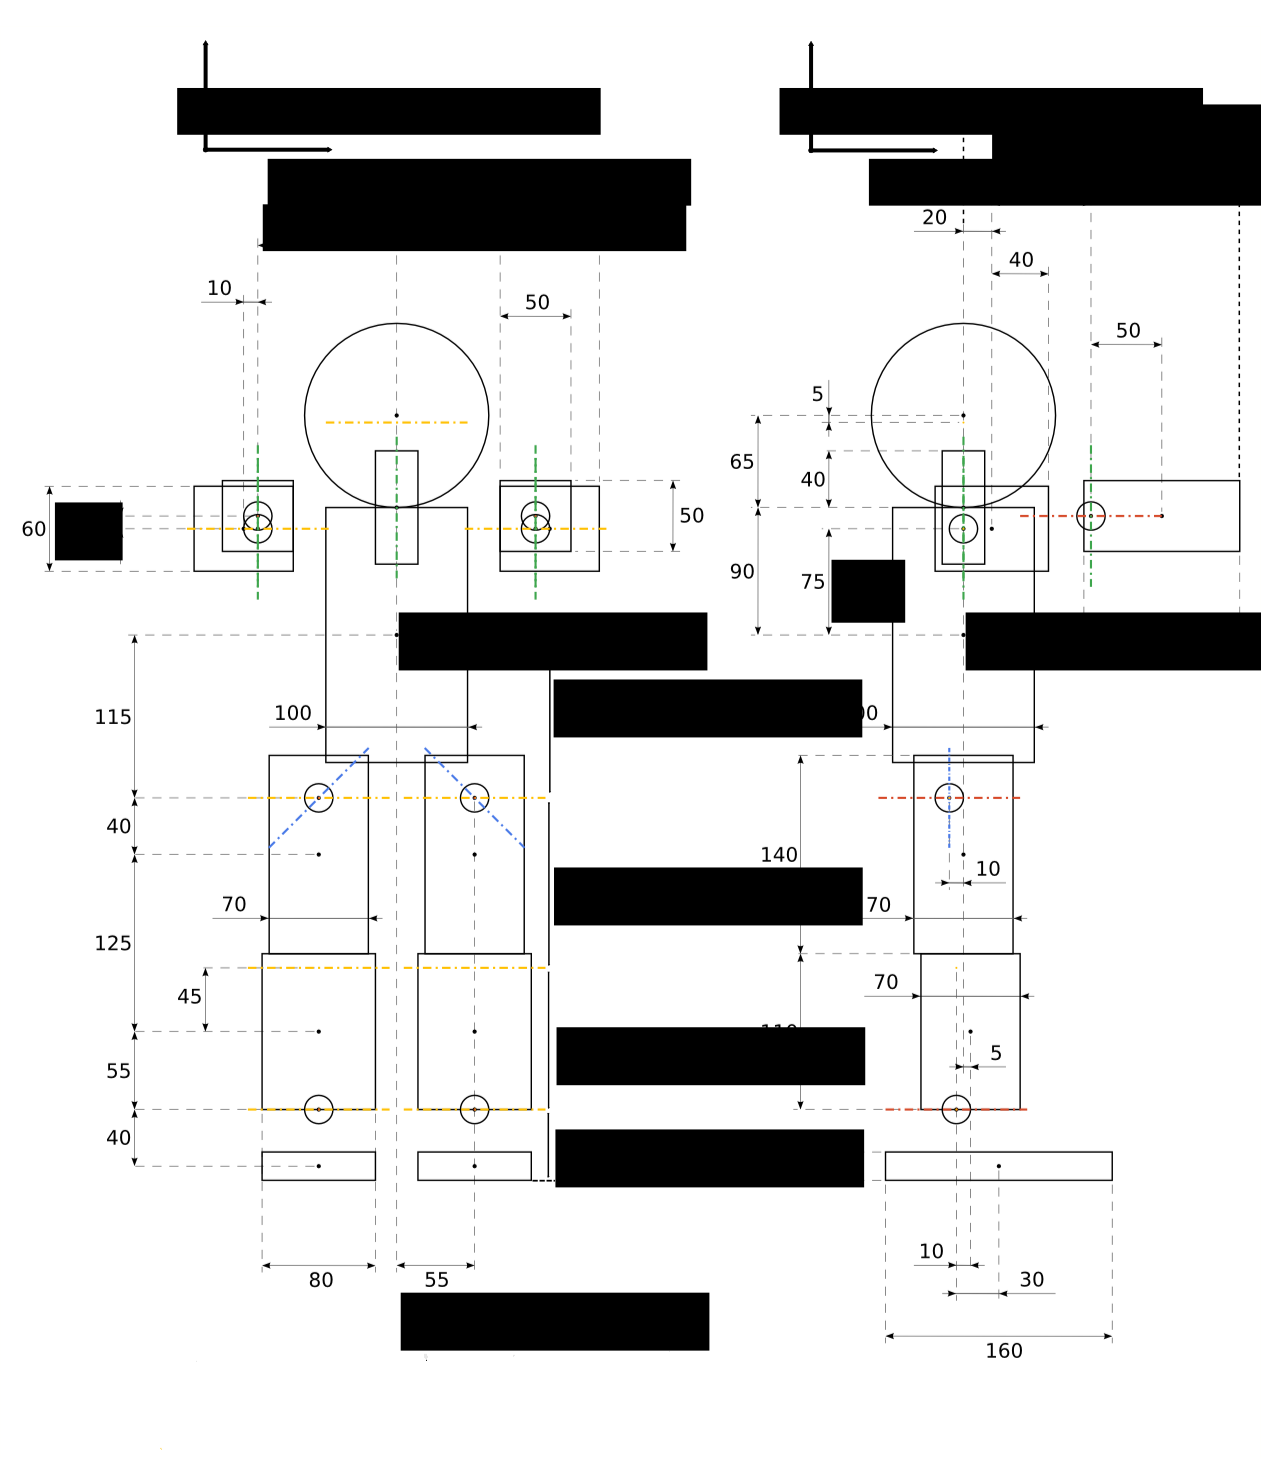
\includegraphics[scale=1.5]{./data/nao_model}
  \caption{Model robota v simulovanej 3D lige \cite{simspark}}
  \label{nao_model}
\end{figure}
\begin{center}
\begin{tabular}{|l|r|}
\hline
\textbf{Končatina} & \textbf{Rozmer (mm)} \\ 
\hline
ShoulderOffsetY	& 98 \\
\hline
ElbowOffsetY & 0 \\
\hline
UpperArmLength & 90 \\
\hline
LowerArmLength & 105 \\
\hline
ShoulderOffsetZ	& 75 \\
\hline
HandOffsetX	& 0 \\
\hline
HandOffsetZ & 9 \\
\hline
HipOffsetZ & 115 \\
\hline
HipOffsetY & 55 \\
\hline
ThighLength	& 120 \\
\hline
TibiaLength	& 100 \\
\hline
FootHeight & 50 \\
\hline
NeckOffsetZ & 90 \\
\hline
\end{tabular}
\end{center}